\chapter{PRELIMINARES Y GENERALIDADES SOBRE CONTROL LQR/LQI}
\label{cap:Notación y preliminares}

El principal propósito de este capítulo es otorgar la introducción sobre las notaciones, definiciones y diseños de control generales utilizados en la Tesis.

\section{Notación} \label{sec:notación}
\lhead[\thepage]{Sección \thesection. Notación}

\subsection{Matrices y vectores} \label{sec:matrices}

Un vector $a\in\mathbb{R}^n$ con notación $\vec{a}$ representa explícitamente un vector con dirección y magnitud en el espacio. En caso que los vectores no representen una dirección, se omite la notación con la flecha superior. Además, para $a\in \mathbb{R}^n$ y $b\in \mathbb{R}^n$ dos vectores, se define el producto cruz entre ambos como $a \times b$. \\

Sea $A \in \mathbb{R}^{n\times n}$ una matriz cuadrada, el radio espectral se define de la forma:
\begin{equation*}
    \rho (A) = \max \{ |\lambda_1|,\ |\lambda_2|,\ \cdots ,\ |\lambda_n| \},
\end{equation*}
donde $\lambda_1, \lambda_2 , \cdots , \lambda_n$ son los autovalores de $A$. El $i$-ésimo valor singular de $A$ se denota como  $\sigma_i(A)$ y el mayor valor singular se define como $\sigma_{\max}(A)$. 

La transpuesta de la matriz $A$ se denota como $A^{\top}$. 

La traza de la matriz $A$ se define como la suma de los elementos de su diagonal principal, es decir:
\begin{equation*}
    \textrm{trace}\left\{ A \right\} = a_{1,1} + a_{2,2} + \hdots + a_{n,n},
\end{equation*}
donde $a_{n,n}$ son los elementos de la $n$-ésima fila y $n$-ésima columna de A. \\

Dada una matriz $B \in \mathbb{R}^{m \times n}$, se define el operador $vec(\cdot)$ de la matriz $B$ como la operación de vectorización (por columnas):
\begin{equation*}
    vec(B)= \left[b_{1,1},\dots ,b_{m,1},b_{1,2},\dots , b_{m,2}, \dots ,b_{1,n}, \dots , b_{m,n} \right]^{\top},
\end{equation*}
donde $b_{m,n}$ son los elementos de la $m$-ésima fila y $n$-ésima columna de la matriz $B$.\\
Sea la variable $v=vec(B) \in \mathbb{R}^{mn}$, al conocer las dimensiones originales de la matriz, es posible reconstruir la matriz $B \in \mathbb{R}^{m \times n}$ aplicando la operación inversa $vec^{-1}(\cdot)$ \cite{magnus1988matrix}. Esta operación inversa es posible calcularla como:
\begin{equation*}
    vec^{-1}(v) = \left( vec(I_n)^{\top} \otimes I_m \right) \left(I_n \otimes v \right),
\end{equation*}
donde $I_n$ e $I_m$ son las matrices identidad de dimensiones $n$ y $m$ respectivamente, y $\otimes$ denota al producto de Kronecker. \\

Sean las matrices $A \in \mathbb{R}^{m\times n}$ y $B \in \mathbb{R}^{p\times q}$, el producto de Kronecker $A \otimes B \in \mathbb{R}^{mp \times nq}$ se define como
\begin{equation*}
    A \otimes B \triangleq \begin{bmatrix} 
    a_{11}B & \cdots & a_{1n}B \\
    \vdots & \ddots & \vdots \\
    a_{m1}B & \cdots & a_{mn}B
    \end{bmatrix},
\end{equation*}
donde $a_{mn} \in \mathbb{R}$ denota el $(m,n)$ elemento de $A$. Se mencionan dos propiedades importantes acerca de el producto de Kronecker a continuación \cite{bernstein2009matrix,horn13,meyer2000matrix}:
\begin{itemize}
    \item Sean $A,B,C,D$ matrices de dimensiones apropiadas, tales que los productos $AC$ y $BD$ están bien definidos, entonces 
    \begin{equation*}
        (A \otimes B) (C \otimes D) = (AC) \otimes (BD).
    \end{equation*}
    \item Sean $A,X,B$ matrices de dimensiones apropiadas, tales que el producto $AXB$ está bien definido, entonces 
    \begin{equation*}
        vec(AXB)= (B^{\top} \otimes A ) vec(X).
    \end{equation*}
\end{itemize}

Sea $A \in \mathbb{R}^{m\times n}$ y $B \in \mathbb{R}^{m\times n}$, se define el producto de Hadamard $A\odot B \in \mathbb{R}^{m \times n}$ como
\begin{equation*}
    A \odot B \triangleq \begin{bmatrix} 
    a_{11} b_{11} & \cdots & a_{1n} b_{1n} \\
    \vdots & \ddots & \vdots \\
    a_{m1}b_{m1} & \cdots & a_{mn}b_{mn}
    \end{bmatrix},
\end{equation*}
donde $a_{mn} \in \mathbb{R}$ denota el $(m,n)$ elemento de $A$ y $b_{mn} \in \mathbb{R}$ denota el $(m,n)$ elemento de $B$ \cite{bernstein2009matrix}.


\subsection{Normas Vectoriales}

\begin{itemize}
    \item Sea $x \in \mathbb{R}^{n}$ un vector, donde el $i$-ésimo elemento de $x$ se denota como $x\{i\}$. Su norma $\norm{x}_p$, con $p \in \mathbb{N}$ se define como
    \begin{align*}
        \norm{x}_p &\triangleq \left( \sum_{i=1}^n \abs{x \{i \}}^p \right)^{1/p}
    \end{align*} 
\end{itemize}

\subsection{Señales}

\begin{itemize}
    \item Dada una señal en tiempo continuo como $x(t)$, cuando el tiempo tiende a infinito, es decir $t \to \infty$, la señal en estado estacionario se denota como $x_\infty$.
\end{itemize}

\section{Control LQR/LQI} \label{sec:lqicontrol}
\lhead[\thepage]{Sección \thesection. Control LQI}

El regulador cuadrático lineal (LQR) es una técnica de control óptimo que busca diseñar un sistema de control que minimice un costo asociado al desempeño de un sistema dinámico. Mediante una función de costo cuadrática, LQR calcula las ganancias óptimas para generar una señal de control que mantenga al sistema estable y eficiente.


\subsection{Regulador Cuadrático Lineal (LQR)}

El control LQR llamado Regulador Cuadrático Lineal, es un tipo de control encargado de regular los estados internos de un sistema dinámico, garantizando estabilidad en el control. La definición del diseño LQR se extrae del libro \textit{Control System Design} \cite{goodwin2001control}. 

Se considera un sistema lineal general definido en variables de estados como:
\begin{subequations} \label{eq:sys_general_varestados}
    \begin{align}
        \Dot{x}(t) & = A x(t) + B u(t), \\
        y(t) & = C x(t) + D u(t)
    \end{align}    
\end{subequations}

Este regulador se caracteriza por ser un control óptimo, debido a que minimiza una función de coste especifica, apreciada en la ecuación siguiente. El diseño se basa en 3 matrices de ponderación ($Q,R,S$), encargadas de la ponderación de los estados, los esfuerzos de control en la entrada y la relación de ambas en el sistema. 

\begin{equation} \label{eq:lqr_funcioncoste}
    J_{LQR} = \int_0^\infty \left( x(t)^{\top} Q x(t) + u(t)^{\top} R u(t) + 2 x(t)^{\top} S u(t)\right) dt,
\end{equation}
donde $Q=Q^{\top}\geq0$, $R=R^{\top}>0$ y $S$ son las matrices de ponderación. 

Una de las formas de resolver el problema de optimización de la función de costo es mediante programación dinámica, como se demuestra en \cite{bertsekas2012dynamic} donde se detalla el proceso de la programación dinámica para funciones de coste. La solución que optimiza que minimiza la función de coste se define como
\begin{equation}
    u^*(t)= -K_x(t) \cdot x(t)
\end{equation}
con $x(t)$ los estados del sistema lineal de \eqref{eq:sys_general_varestados} y la matriz $K_x(t)$ de realimentación de los estados definida como

\begin{equation}
    K_x(t) = R^{-1} B^{\top} P(t)
\end{equation}

donde $P(t)$ es la solución a la ecuación diferencial de Riccati de tiempo continuo
\begin{equation}
    -\dot{P}(t) = A^{\top} P(t) + P(t) A - P(t) B R^{-1} B^{\top} P(t) + Q
\end{equation}
con $A,B,C$ matrices del sistema lineal en variables de estados. 

Si el sistema $(A,B)$ es estabilizable y los estados son detectables, se tiene que para $t \to \infty$ la solución de la ecuación diferencial de Riccati converge a un estado estacionario $P_\infty$. 

\begin{mybox}{}
    \begin{lemma} \label{lem1:riccati_infinto}
        Si P(t) converge en $t \to \infty$, su valor en estado estacionario $P_\infty$ satisface la siguiente ecuación algebraica de Riccati para tiempo continuo \cite{goodwin2001control}:
        \begin{equation}
            0 = A^{\top} P_\infty + P_\infty A - P_\infty B R^{-1} B^{\top} P_\infty + Q
        \end{equation}
        Con el valor estacionario $P_\infty$ de la ecuación de Riccati en tiempo continuo, entonces es posible definir un control óptimo estable del sistema como:
        \begin{equation}
            u^*(t) = - K_{x_\infty} x(t)
        \end{equation}
         donde $K_{x_\infty} = R^{-1} B^{\top} P_\infty$
    \end{lemma}
\end{mybox}

\begin{proof}
    La demostración del Lema \ref{lem1:riccati_infinto} se encuentra en \cite{goodwin2001control}.
\end{proof}

En la Figura \ref{fig:lqr_scheme} se puede apreciar el esquema de control LQR para la planta $G$, con $u$, $x$ e $y$ la actuación, los estados y la salida de la planta respectivamente.

\begin{figure}[ht]
\centering
    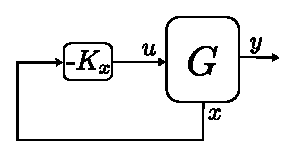
\includegraphics[width=0.4\columnwidth]{Figures/Preliminares/lqr_scheme.eps}
    \caption{Esquema de control LQR.}
    \label{fig:lqr_scheme}
\end{figure}

El requisito principal para el diseño de control LQR es tener disponibles los estados internos del sistema. El problema radica en que no siempre estos estados estarán disponibles y/o medibles en la salida del sistema. Para solucionar esto es posible utilizar un observador de Luenberger (o un filtro de Kalman si se está en presencia de ruidos gaussianos) el cual se encarga de estimar los estados del sistema \cite{skogestad2005multivariable}.

El control óptimo LQR está enfocado en la regulación de estados, no así en el seguimiento de referencia como tal. Es por esto que mediante el principio del modelo interno es posible incluir un estado extra encargado de el seguimiento de la referencia como se define en el diseño de control LQI a continuación.

\subsection{Control Integral Cuadrático Lineal (LQI)}

Mediante una acción integral es posible incluir el seguimiento de referencia en el problema de regulación manteniendo un diseño de control optimo \cite{feng2007lqi}.

Sea el sistema lineal \eqref{eq:sys_general_varestados} en variables de estados, considerando $D$ cero, la referencia $r$ a seguir del sistema y la salida medible $y$, se define el error de seguimiento como:
\begin{align}
    e(t) & = r(t) - y(t) \notag \\
    & = r(t) - C x(t)
\end{align}

Se establece un estado aumentado del sistema, en donde se incluye la integral del error como un estado extra.

\begin{equation}
    z(t) = \begin{bmatrix}
        x(t) \\ \int e(t)
    \end{bmatrix} 
    = \begin{bmatrix}
        x(t) \\ x_i(t)
    \end{bmatrix}
\end{equation}

Se describe el sistema aumentado en variables de estados de la forma:

\begin{equation}
    \begin{bmatrix}
        \dot{x}(t) \\ \dot{x}_i(t)
    \end{bmatrix} = \underbrace{\begin{bmatrix}
        A & 0 \\ -C & 0 
    \end{bmatrix}}_{A_a} \begin{bmatrix}
        x(t) \\ x_i(t)
    \end{bmatrix} + \underbrace{\begin{bmatrix}
        B \\ 0
    \end{bmatrix}}_{B_a} u(t) + \begin{bmatrix}
        0 \\ I
    \end{bmatrix} r(t)
\end{equation}
donde $I$ es la matriz identidad de dimensión apropiada. 

Dado que se busca que el sistema en estado estacionario cumpla $\dot{x}_\infty = A x_\infty + B u_\infty$ y que $\dot{x}_{i_\infty} = e_\infty  = 0$, el sistema aumentado anterior es equivalente a:

\begin{equation} \label{eq:sys_aumentado_lqi}
    \begin{bmatrix}
        \dot{x}(t) \\ \dot{x}_i(t)
    \end{bmatrix} = \underbrace{\begin{bmatrix}
        A & 0 \\ -C & 0 
    \end{bmatrix}}_{A_a} \begin{bmatrix}
        x(t) \\ x_i(t)
    \end{bmatrix} + \underbrace{\begin{bmatrix}
        B \\ 0
    \end{bmatrix}}_{B_a} u(t)
\end{equation}

Con el sistema aumentado, el diseño de control se traduce en un control LQR para el estado aumentado $z(t)=\begin{bmatrix} x(t)^{\top} & x_i(t)^{\top} \end{bmatrix}^{\top}$.

La función de coste asociada al problema de control LQI es:
\begin{equation} \label{eq:lqi_funcioncoste}
    J_{LQI} = \int_0^\infty \left( z(t)^{\top} Q z(t) + u(t)^{\top} R u(t) + 2 z(t)^{\top} S u(t)\right) dt,
\end{equation}
donde $Q=Q^{\top}\geq0$, $R=R^{\top}>0$ y $S$ son las matrices de ponderación del estado aumentado, del esfuerzo de control en la entrada, y de la relación entre ambos elementos.

La solución óptima al funcional de costo asociado es:
\begin{equation}
    u^*(t) = -K_x x(t) - K_i x_i(t)
\end{equation}
donde 
\begin{equation}
    \begin{bmatrix}
        K_x & K_i 
    \end{bmatrix} = R^{-1} B_a^{\top} P_\infty
\end{equation}
con $P_\infty$ la solución a la ecuación algebraica de Riccati en tiempo continuo dada por:
\begin{equation}
    0 = A_a^{\top} P_\infty + P_\infty A_a - P_\infty B_a R^{-1} B_a^{\top} P_\infty + Q
\end{equation}
con las matrices $A_a$ y $B_a$ del sistema aumentado \eqref{eq:sys_aumentado_lqi}.

El control LQI logra una solución estable y óptima respecto al funcional de costo asociado, además de garantizar error de seguimiento cero en estado estacionario para señales de referencias de tipo escalón \cite{young1972approach}.

En la Figura \ref{fig:lqi_scheme} se ilustra el esquema de control LQI para la referencia $r$, con $u$, $x$ e $y$ la actuación, los estados y la salida de la planta $G$ respectivamente.

\begin{figure}[ht]
\centering
    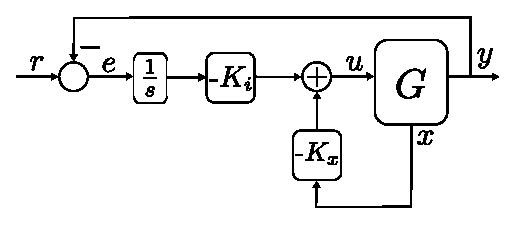
\includegraphics[width=0.6\columnwidth]{Figures/Preliminares/lqi_scheme.eps}
    \caption{Esquema de control LQI.}
    \label{fig:lqi_scheme}
\end{figure}



\newpage
\section{Output Regulation} \label{sec:outputregulation}
\lhead[\thepage]{Sección \thesection. Output Regulation}

El desarrollo conceptual y teórico del problema Output Regulation es obtenido directamente desde el libro \textit{Nonlinear Output Regulation: Theory and Applications} \cite{huang2004bookoutputregulation}.

Sea el sistema lineal general con perturbación, descrito en variables de estados de la forma:

\begin{subequations} \label{eq:sys_general_outputregulation}
    \begin{align}
        \Dot{x}(t) & = A x(t) + B u(t) + E_d d(t), \quad x(0) = x_0, \quad t \geq 0,\\
        y(t) & = C x(t) + D u(t) + F_d d(t),\\
        e(t) & = C x(t) + D u(t) + F_d d(t) - r(t)
    \end{align}    
\end{subequations}

donde $x(t)$ es el estado $n$-dimensional del sistema, $u(t)$ la entrada $m$-dimensional del sistema, $r(t)$ la referencia deseada, $e(t)$ el error de seguimiento y $d(t)$ la perturbación.

La referencia y la perturbación se suponen que son generadas por ecuaciones diferenciales autónomas lineales, con $r_0$ y $d_0$ estados iniciales arbitrarios:
\begin{equation}
    \dot{r}(t) = A_{1r} r(t), \quad r(0)=r_0, \qquad \dot{d}(t) = A_{1d} d(t), \quad d(0)=d_0
\end{equation}

Así, se definen las señales exógenas compuestas por la referencia y la perturbación del sistema como un exosistema:
\begin{equation}
    \dot{v}(t) = A_1 v(t), \quad v(0) = v_0, \quad t \geq 0 
\end{equation}
donde
\begin{equation*}
    v(t) =\begin{bmatrix} r(t) \\ d(t) \end{bmatrix}, \quad A_1 = \begin{bmatrix} A_{1r} & 0 \\ 0 & A_{1d} \end{bmatrix}, \quad v_0 \overset{def}{=} \begin{bmatrix} r_0 \\ d_0 \end{bmatrix}
\end{equation*}

Con esto, se reescribe por conveniencia el sistema lineal \eqref{eq:sys_general_outputregulation} en un sistema lineal compuesto dado por:
\begin{subequations} \label{eq:sys_compuesto_outputregulation}
    \begin{align}
        \Dot{x}(t) & = A x(t) + B u(t) + E v(t),\\
        \dot{v}(t) & = A_1 v(t), \\ 
        e(t) & = C x(t) + D u(t) + F v(t)
    \end{align}    
\end{subequations}

con $v(t)$ la señal exógena $q$-dimensional, $\begin{bmatrix} E \\ F \end{bmatrix} = \begin{bmatrix} 0 & E_d \\ -I & F_d \end{bmatrix}$, e $I$ la matriz identidad.

Sea la ley de control caracterizada por la realimentación de estados del sistema:

\begin{equation} \label{eq:lawcontrol_outputregulation}
    u(t) = K_x x(t) + K_v v(t),
\end{equation}
donde las matrices $K_x \in \mathcal{R}^{m\times n}$ y $K_v \in \mathcal{R}^{m\times q}$ son ganancias constantes.

Considerando el sistema lineal compuesto \eqref{eq:sys_compuesto_outputregulation} (que incluye a la planta y al exosistema mencionados anteriormente), junto a la ley de control \eqref{eq:lawcontrol_outputregulation}, podemos describir el sistema en lazo cerrado como:
\begin{subequations} \label{eq:sys_acl_outputregulation}
    \begin{align}
        \dot{x}_c (t) & = A_c x_c(t) + B_c v(t), \qquad x_c(0) = x_{c0}, \\
        \dot{v}(t) & = A_1 v(t), \\
        e(t) & = C_c x_c(t) + D_c v(t)
    \end{align}
\end{subequations}

donde las matrices de lazo cerrado son:
\begin{align}
    A_c & = A + B K_x, \qquad B_c = E + B K_v, \notag \\
    C_c & = C + D K_x, \qquad D_c = F + D K_v 
\end{align}

Se introduce la siguiente definición para describir los requerimientos de Output Regulation.
\begin{mybox}{}
    \begin{definition} \label{def1:acl_outputregulation}
        El sistema en lazo cerrado \eqref{eq:sys_acl_outputregulation} se dice exponencialmente estable si cumple las siguientes propiedades:
        \begin{enumerate}[leftmargin=*, labelindent=1em, label=\textbf{Propiedad \thedefinition.\arabic*}]
            \item \label{def_prop1.1} La matriz $A_c$ es Hurwitz, es decir, todos los autovalores de $A_c$ tienen parte real negativa (son estables). Además la matriz $A_1$ no posee partes reales negativas.
            \item \label{def_prop1.2} Para cualquier valor inicial de $x_{c0}$ y $v_0$ la trayectoria del sistema compuesto \eqref{eq:sys_compuesto_outputregulation} satisface:
            \begin{equation}
                \lim_{t\to \infty} e(t) = \lim_{t \to \infty} (C_c x_c(t)+D_c v(t)) = 0
            \end{equation}
        \end{enumerate}
        La ley de control del sistema en lazo cerrado debe satisfacer ambas propiedades descritas para resolver el problema lineal de Output Regulation.
    \end{definition}
\end{mybox}

\begin{assumption}
\label{assum1:regulation_assumption}
    Bajo la definición \ref{def1:acl_outputregulation} anterior, se asumen 3 condiciones para resolver el problema lineal de Output Regulation:
    \begin{enumerate}[leftmargin=*, labelindent=1em, label=\textbf{(\theassumption.\alph*)}]
        \item \label{assum1.1} $A_1$ no posee autovalores con parte real negativa. 
        \item \label{assum1.2} El par $(A,B)$ es estabilizable. 
        \item El par $\left( \begin{bmatrix} C & F \end{bmatrix}, \begin{bmatrix} A & E \\ 0 & A_1 \end{bmatrix} \right)$ es detectable.
    \end{enumerate}
\end{assumption}

\begin{mybox}{}
    \begin{lemma} \label{lem2:regulation_equation}
        Bajo la suposición \ref{assum1.1} y considerando la ley de control \eqref{eq:lawcontrol_outputregulation}, se asume que el sistema en lazo cerrado \eqref{eq:sys_acl_outputregulation} posee la \ref{def_prop1.1}. Entonces, las siguientes declaraciones son equivalentes:
        \begin{enumerate}
            \item El sistema en lazo cerrado posee la \ref{def_prop1.2}. 
            \item El controlador resuelve el problema lineal Output Regulation.
            \item Existe una única matriz $X_c$ que satisface las siguientes ecuaciones matriciales:
            \begin{align} \label{eq:lem2_eqRegulation}
                X_c A_1 = A_c X_c + B_c \notag \\
                0 = C_c X_c + D_c
            \end{align}
        \end{enumerate}
        \begin{remark}
            Resolución del sistema de ecuaciones \ref{eq:lem2_eqRegulation} demostrado en Apéndice \ref{appen1}.
        \end{remark}
    \end{lemma}
\end{mybox}

Bajo la siguiente transformación lineal es posible obtener un mejor enfoque de resolución del problema Output Regulation:
\begin{equation}
    \begin{bmatrix}
        X \\ U
    \end{bmatrix} = \begin{bmatrix}
        I_n & 0_{n\times m} \\ K_x & I_m
    \end{bmatrix} 
    \begin{bmatrix}
        X_c \\ K_v    
    \end{bmatrix}
\end{equation}

\begin{mybox}{}
    \begin{theorem} \label{teo1:OutputRegulation}
        Bajo las suposiciones \ref{assum1.1} y \ref{assum1.2}, se establece la ganancia de realimentación de control $K_x$ tal que $(A+BK_x)$ es exponencialmente estable. Luego, el problema lineal Output Regulation se puede resolver por la ley de control de realimentación de estados:
        \begin{equation}
            u(t) = K_x x(t) + K_v v(t)
        \end{equation}
        si y solo si existen 2 matrices $X$ y $U$ tales que satisfagan las ecuaciones matriciales de regulación:
        \begin{align}\label{eq:teo1_eqRegulation}
            X A_1 = A X + B U + E \notag \\
            0 = C X + D U + F
        \end{align}
                
        con la ganancia de realimentación $K_v$ dada por la transformación lineal:
        \begin{equation}
            K_v = U - K_x X
        \end{equation}
        donde las matrices $A,B,C,D,E,F$ y $A_1$ están determinadas por la planta y la referencia a seguir. 
        \begin{remark}    
         Resolución del sistema de ecuaciones \eqref{eq:teo1_eqRegulation} demostrado en Apéndice \ref{appen1}.
         \end{remark}
    \end{theorem}
\end{mybox}

En la Figura \ref{fig:output_regulation_scheme} se ilustra el esquema de control LQR Output Regulation, donde $v$ es la referencia, y $u$, $x$ e $y$ son la actuación, los estados y la salida de la planta $G$ respectivamente.

\begin{figure}[ht]
\centering
    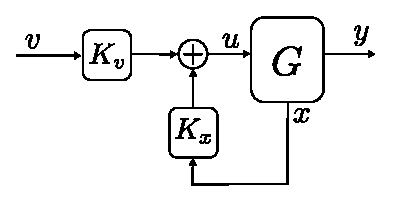
\includegraphics[width=0.45\columnwidth]{Figures/Preliminares/output_regulation_scheme.eps}
    \caption{Esquema de control LQR Output Regulation.}
    \label{fig:output_regulation_scheme}
\end{figure}
